%======================================================================
\section{Steady rolls and the construction questions}\label{sec:steady}
%======================================================================

Both halves of item~3 ask, in different words, whether some solution comes close to the proven bound. A natural
place to look is among steady rolls. They are exact solutions at every Rayleigh number, they are what a
computer-assisted existence proof would naturally target, and at $\mathrm{Pr}=1$ the Nusselt-maximising rolls are
known numerically to reach the classical $\mathrm{Ra}^{1/3}$ scaling \citep{WenGoluskinDoering2022}. Steady rolls
at large Rayleigh number have been computed between no-slip walls for $1\le\mathrm{Pr}\le100$
\citep{SondakSmithWaleffe2015,WenGoluskinDoering2022} and between stress-free walls
\citep{ChiniCox2009,WenEtAl2020,WenEtAl2026}. Steady cells at infinite Prandtl number have a long history in
boundary-layer theory \citep{Roberts1979,JimenezZufiria1987}, but we did not find a study of the Nusselt-maximising
period between no-slip walls at infinite Prandtl number. We therefore
computed, at infinite Prandtl number and in two dimensions, the steady mirror-symmetric rolls that are extremal
over the horizontal period $\Gamma$ at each Rayleigh number. These are $F_B$-minimising rolls for internally heated
convection and $\mathrm{Nu}$-maximising rolls for Rayleigh--B\'enard convection, both with no-slip walls.

\paragraph{Method.} Starting near onset, we continue in $\log_{10}R$ in steps of $0.25$. At each step a
golden-section search over $\log\Gamma$, to tolerance $0.01$, locates an optimum, with every evaluation a Newton
solve from the nearest stored solution. Resolution rises with $R$, from $(N_z,N_x)=(32,32)$ to $(80,72)$ per
period, and to $(96,96)$ above $\mathrm{Ra}=3\times10^7$. Re-solving at $(112,104)$ changes Nu at
$\mathrm{Ra}=10^7$ by $4\times10^{-7}$ (relative) and $F_B$ at $R=1.6\times10^7$ by $10^{-10}$; re-solving at
$(128,128)$ changes Nu at $\mathrm{Ra}=5.6\times10^7$ and $10^8$ by $5\times10^{-6}$ and $2\times10^{-5}$
(Table~\ref{tab:steady}). For $\mathrm{Ra}\ge10^6$ the coefficients in the last tenth of the stored Fourier
spectrum are below $10^{-10}$ of the largest coefficient. The Chebyshev tails are below $10^{-8}$ for internally
heated rolls and below $4\times10^{-5}$ for Rayleigh--B\'enard rolls, whose thermal boundary layers are thinner;
the re-solves show the error in Nu to be no larger than that tail. Golden-section search follows a \emph{local}
optimum. We therefore also mapped $\mathrm{Nu}(\Gamma)$ along the roll family by continuation in $\Gamma$, at
fixed $\mathrm{Ra}=10^5$, $1.8\times10^5$, $3.2\times10^5$, $5.6\times10^5$, $10^6$ and $10^7$, and $F_B(\Gamma)$
at $R=1.6\times10^6$. At $\mathrm{Ra}=10^5$ this revealed a second, slightly higher maximum that the local search
had missed. Table~\ref{tab:steady} and Figure~\ref{fig:steady} report the largest maximum found over the scanned
period range. All statements below concern this mirror-symmetric, layer-spanning roll family and the sampled
Rayleigh numbers and periods; we did not search over other steady solutions.

\paragraph{Internally heated convection.} The $F_B$-minimising rolls obey
$F_B\approx1.29\,R^{-0.093}$ for $1.6\times10^6\le R\le2.8\times10^7$ (six Rayleigh numbers), with
$\Gamma^*\approx12.4R^{-0.21}$ (Table~\ref{tab:steady}, Figure~\ref{fig:steady}a). The fitted exponent depends
mildly on the range: $-0.0915$ from $R\ge1.6\times10^5$ and $-0.097$ from the last two points alone. Such fits
describe the computed range; they do not establish an asymptotic exponent. For $R\ge8\times10^5$ the fluxes lie
$1$--$4\%$ \emph{below} the time-dependent values of \citet{ArslanRojas2025} at the same $R$ (interpolated), and
the exponent is close to theirs, $-0.092$. At lower $R$, where their data scatter, the steady values are up to
$11\%$ higher. At $R=1.6\times10^6$, $F_B(\Gamma)$ increases monotonically on both sides of the optimum: down to
$\Gamma\approx0.26$, where the roll family meets the conduction state ($F_B=\frac12$), and up to $\Gamma=1$.
Steady rolls of this family therefore come only marginally closer to the bound than the time-dependent flows do.
At $R=2.8\times10^7$ they sit a factor of $115$ above the unconditional bound of Corollary~\ref{cor:R} (with
$\mathcal T_{\max}=1.29$ for their period), and a factor of $49$ above the conditional bound with
$\mathcal T=1/8$. Their maximum
temperature falls with $R$, roughly as $R^{-0.21}$ (from $0.123$ at $R=5\times10^4$ to $0.035$ at
$R=2.8\times10^7$). With this measured $\mathcal T$ the bound evaluated on the rolls scales as about $R^{-0.30}$,
still far below their $R^{-0.093}$.

\paragraph{Rayleigh--B\'enard convection at infinite Prandtl number.} Near onset $\mathrm{Nu}(\Gamma)$ has a
single maximum, on a branch of wide rolls whose period shrinks roughly as $\mathrm{Ra}^{-1/5}$: $\Gamma^*=1.67$ at
$\mathrm{Ra}=10^4$ and $1.04$ at $\mathrm{Ra}=10^5$, so that $\Gamma^*\mathrm{Ra}^{1/5}$ stays between $10.4$ and
$10.6$. At $\mathrm{Ra}=10^5$ a second maximum has appeared, at narrower rolls ($\Gamma=0.744$), with Nu only
$0.013\%$ below the wide-roll value ($4.79376$ against $4.79437$; neither changes by more than $10^{-8}$,
relative, between $N_z=48$ and $64$). By $\mathrm{Ra}=1.8\times10^5$ the wide-roll maximum is not detected in the scans: $\mathrm{Nu}(\Gamma)$
decreases monotonically from the narrow optimum up to the largest period scanned, $\Gamma\approx1.8$ for
$1.8\times10^5\le\mathrm{Ra}\le5.6\times10^5$, $1.20$ at $\mathrm{Ra}=10^6$ and $0.91$ at $\mathrm{Ra}=10^7$
(Figure~\ref{fig:steady}c). From then on the largest maxima found are narrow rolls. They follow
\[
\mathrm{Nu}\approx0.153\,\mathrm{Ra}^{0.298},\qquad \Gamma^*\approx11.7\,\mathrm{Ra}^{-0.249}
\qquad(10^6\le\mathrm{Ra}\le10^8),
\]
with local exponents of $0.298$--$0.299$ over the last nine steps (Figure~\ref{fig:steady}b); fitting from
$\mathrm{Ra}\ge10^5$ or from $\mathrm{Ra}\ge10^7$ gives $0.2979$ and $0.2986$. At
$\mathrm{Ra}=10^6$, for instance, $\mathrm{Nu}=9.46$ at the optimum $\Gamma=0.37$ and $8.52$ at $\Gamma=1.04$,
whereas at $\mathrm{Pr}=1$ the optimum reported by \citet{WenGoluskinDoering2022} is $\mathrm{Nu}=10.39$ at
$\Gamma=0.88$.

This is the high-wavenumber regime $\Gamma=c\,\mathrm{Ra}^{-1/4}$. For stress-free walls the matched asymptotics
of \citet{WenEtAl2026} predict $\mathrm{Nu}=O(\mathrm{Ra}^{3/10})$, their most nearly asymptotic data give an
exponent of $0.298$, and they suggest that the same scaling holds between no-slip walls. Our no-slip rolls at
infinite Prandtl number support that suggestion. The switch from wide to narrow optima continues a trend that
\citet{SondakSmithWaleffe2015} found for no-slip rolls at $\mathrm{Pr}=1$, $4$, $7$, $10$ and $100$: for
$\mathrm{Pr}\le7$ the wide-roll maximum stays the larger one over their range, whereas for $\mathrm{Pr}=10$ and
$100$ the narrow-roll maximum eventually overtakes it. (They report $\mathrm{Nu}\sim\mathrm{Ra}^{0.31}$ for their optimal rolls, with
at most a very weak dependence of the exponent on Pr.) At $\mathrm{Pr}=1$ the wide-roll maximum, with $\Gamma^*=O(\mathrm{Ra}^{-1/5})$, gives
$\mathrm{Nu}\sim\mathrm{Ra}^{1/3}$ \citep{WenGoluskinDoering2022}. At infinite Prandtl number it is not merely
overtaken: from $\mathrm{Ra}=1.8\times10^5$ onwards it is not detected within the periods we scanned.

The wide-roll maximum leaves a trace. Beyond the optimum the local slope $d\ln\mathrm{Nu}/d\ln\Gamma$ has a shallow
extremum, a shoulder (Figure~\ref{fig:steady}d). Its slope is $-0.012$ at $\mathrm{Ra}=1.8\times10^5$,
$-0.030$ at $3.2\times10^5$, $-0.049$ at $5.6\times10^5$, $-0.067$ at $10^6$ and $-0.115$ at $10^7$. Its position,
$\Gamma\mathrm{Ra}^{1/5}=10.0$--$10.4$, continues the line on which the wide-roll optimum lay for
$\mathrm{Ra}\le10^5$. The $\mathrm{Pr}=1$ optimum follows the same scaling, at
$\Gamma\mathrm{Ra}^{1/5}=13.6$--$13.9$ for $10^6\le\mathrm{Ra}\le10^7$ in the table of
\citet{WenGoluskinDoering2022}. So the shoulder is the remnant of the wide-roll maximum, and it moves steadily
further from being a maximum as Ra grows. Together with the Prandtl-number trend of
\citet{SondakSmithWaleffe2015}, this suggests that inertia is what sustains that maximum at finite Prandtl number;
we have not tested that suggestion directly. Our scans cannot exclude a reversal of the trend at much higher Ra,
or a maximum at periods beyond those scanned.

\paragraph{Consequence for the construction question.} If these trends persist, a computer-assisted
construction based on two-dimensional steady rolls of this family will not reach
$\mathrm{Nu}\ge c\,\mathrm{Ra}^{1/3}$ at infinite Prandtl number. An asymptotic $3/10$ law, if established, would lose a factor
$\mathrm{Ra}^{1/30}$ relative to $\mathrm{Ra}^{1/3}$; the present finite-range fit does not establish that law.
This is consistent with the heuristic that a single-scale roll at infinite Prandtl number is limited by the
interior elevator balance. Narrow cells need an interior temperature gradient $\beta\simeq k^4/\mathrm{Ra}$ to
convect. Matching the interior flux $k^2A^2/\mathrm{Ra}$ (for vertical velocity amplitude $A$) to a wall layer of
L\'ev\^eque type, $\mathrm{Nu}\sim(Ak^2)^{1/3}$, gives $\mathrm{Nu}\sim\mathrm{Ra}^{1/5}k^{2/5}$. This is maximal
at the largest admissible wavenumber $k\sim\mathrm{Ra}^{1/4}$, where $\mathrm{Nu}\sim\mathrm{Ra}^{3/10}$. The
classical exponent then requires structure on several scales, such as near-wall cells of width
$\mathrm{Ra}^{-1/3}$ that coarsen into the interior. Optimal-transport ``branching'' flows have this structure
\citep{TobascoDoering2017}. They are not known to arise as solutions of the infinite-Prandtl Boussinesq equations,
and constructing one, steady or not, in two or three dimensions, remains the open problem. Our finite scans motivate this question; they do not establish an obstruction theorem or exclude disconnected branches.

\begin{table}[t]\centering\footnotesize
\caption{Extremal steady rolls at infinite Prandtl number, no-slip walls ($d=2$). Left: internally heated,
$F_B$-minimising period $\Gamma^*$. Right: Rayleigh--B\'enard, Nu-maximising period. Resolution $N_z,N_x$ is per
period. $^\dagger$Largest maximum found by continuation in $\Gamma$ (Section~\ref{sec:steady}); the narrow-roll
local maximum at this Rayleigh number is $\mathrm{Nu}=4.79376$ at $\Gamma=0.7440$.}\label{tab:steady}
\setlength{\tabcolsep}{3.5pt}
\begin{tabular}{lcccc|lccc}\hline
\multicolumn{5}{c|}{internally heated} & \multicolumn{4}{c}{Rayleigh--B\'enard}\\
$R$ & $N_z,N_x$ & $\Gamma^*$ & $F_B$ & $\mathcal T$ & Ra & $N_z,N_x$ & $\Gamma^*$ & Nu\\\hline
$5.00\times10^{4}$ & 48, 40 & 1.5083 & 0.47694 & 0.1232 & $10^{4}$ & 32, 32 & 1.6655 & 2.62770 \\
$8.89\times10^{4}$ & 48, 40 & 1.2719 & 0.44386 & 0.1116 & $1.78\times10^{4}$ & 32, 32 & 1.4887 & 3.06821 \\
$1.58\times10^{5}$ & 48, 40 & 1.0840 & 0.41770 & 0.1001 & $3.16\times10^{4}$ & 32, 32 & 1.3306 & 3.56010 \\
$2.81\times10^{5}$ & 48, 40 & 0.9323 & 0.39523 & 0.0894 & $5.62\times10^{4}$ & 48, 40 & 1.1894 & 4.12900 \\
$5.00\times10^{5}$ & 64, 56 & 0.8138 & 0.37506 & 0.0799 & $10^{5}$ & 64, 152 & 1.0361$^\dagger$ & 4.79437 \\
$8.89\times10^{5}$ & 64, 56 & 0.7143 & 0.35639 & 0.0713 & $1.78\times10^{5}$ & 48, 40 & 0.5964 & 5.66079 \\
$1.58\times10^{6}$ & 64, 56 & 0.6301 & 0.33872 & 0.0636 & $3.16\times10^{5}$ & 48, 40 & 0.5050 & 6.71227 \\
$2.81\times10^{6}$ & 64, 56 & 0.5567 & 0.32172 & 0.0566 & $5.62\times10^{5}$ & 64, 56 & 0.4332 & 7.96769 \\
$5.00\times10^{6}$ & 80, 72 & 0.4923 & 0.30525 & 0.0503 & $10^{6}$ & 64, 56 & 0.3732 & 9.46001 \\
$8.89\times10^{6}$ & 80, 72 & 0.4361 & 0.28928 & 0.0447 & $1.78\times10^{6}$ & 64, 56 & 0.3228 & 11.23201 \\
$1.58\times10^{7}$ & 80, 72 & 0.3878 & 0.27383 & 0.0397 & $3.16\times10^{6}$ & 64, 56 & 0.2792 & 13.33574 \\
$2.81\times10^{7}$ & 80, 72 & 0.3458 & 0.25894 & 0.0352 & $5.62\times10^{6}$ & 80, 72 & 0.2421 & 15.83368 \\
 & & & &  & $10^{7}$ & 80, 72 & 0.2094 & 18.80013 \\
 & & & &  & $1.78\times10^{7}$ & 80, 72 & 0.1816 & 22.32351 \\
 & & & &  & $3.16\times10^{7}$ & 80, 72 & 0.1574 & 26.50982 \\
 & & & &  & $5.62\times10^{7}$ & 96, 96 & 0.1365 & 31.48225 \\
 & & & &  & $10^{8}$ & 96, 96 & 0.1184 & 37.39233 \\
\hline
\multicolumn{5}{l|}{Resolution check} & \multicolumn{4}{l}{Resolution check}\\
$1.58\times10^{7}$ & 80, 72 & & 0.27382701 &  & $10^{7}$ & 80, 72 & & 18.800132 \\
$1.58\times10^{7}$ & 112, 104 & & 0.27382701 &  & $10^{7}$ & 112, 104 & & 18.800124 \\
 & & & &  & $5.62\times10^{7}$ & 128, 128 & & 31.482426 \\
 & & & &  & $10^{8}$ & 128, 128 & & 37.391696 \\
\hline\end{tabular}\end{table}


\begin{figure}[t]\centering
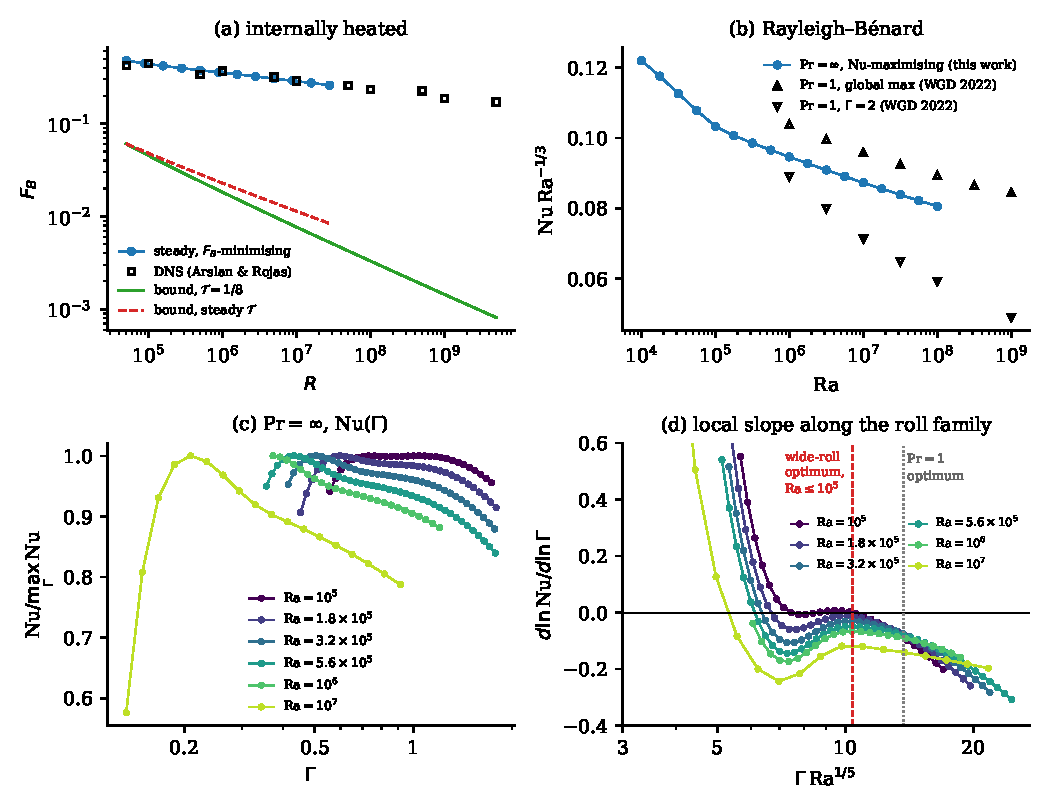
\includegraphics[width=\textwidth]{fig4_steady.pdf}
\caption{Steady rolls at infinite Prandtl number, no-slip walls. (a) Internally heated: $F_B$ of
$F_B$-minimising rolls, the time-dependent simulations of \citet{ArslanRojas2025}, and \eqref{eq:mainbound}
with $\mathcal T=1/8$ (conditional) and with the rolls' own maximum temperature. (b) Rayleigh--B\'enard: $\mathrm{Nu}\,\mathrm{Ra}^{-1/3}$ for Nu-maximising rolls,
compared with the $\mathrm{Pr}=1$ rolls of \citet{WenGoluskinDoering2022}. (c) $\mathrm{Nu}(\Gamma)$ along the roll
family at fixed Ra, normalised by its maximum. (d) The local slope of (c) against $\Gamma\mathrm{Ra}^{1/5}$. Dashed: the line
$\Gamma\mathrm{Ra}^{1/5}=10.4$ on which the wide-roll optimum lies for $\mathrm{Ra}\le10^5$; dotted: the
$\mathrm{Pr}=1$ optimum of \citet{WenGoluskinDoering2022}.}\label{fig:steady}
\end{figure}
